\chapter{Methods}

\begin{comment}
  <blockquote>
Methodik, die verfolgt wurde, um Lösung zu entwickeln
 -> ich glaube, den Hevner Artikel (Design Science in Inf Sys research) habe ich dir eh geschickt, eignet sich als Methode. Verbinde einfach sein abstraktes Konzept mit dem, was du tatsächliche gemacht hast (was war die Ausgangssituation (Legacy code mit Angular), wie hat dein Suchprozess ausgesehen (wie bist du auf react gekommen, was waren die Alternativen,...), Was kam aus der globalen Knowledge Base (react), wie kamst du zu deiner Synthese aus react+rdfstore-js+angular)
 </blockquote>

 <blockquote>
 in the method chapter you should explain:
* hevner
* RDF, linked data, JSON-LD
* angular
* flux/redux
 </blockquote>

 % Flo @ hevner-summary: good first note sheet. You can convert that into a 1-2 page intro of the methods section. Then you go on to show how you applied this framework, effectively proving that what you did is research, and not engineering.

 % TODO better describe/address the figure

% 2: @hevner-länge: macht nichts, aber man darf sich beim lesen nicht fragen, warum du einem das erzählstFrom:phlow_06 (Flo SAT)wenn du keinen grund dafür findest: weglassen. sonst: sagen. -- dh ich sollte e.g. auch nur die artefakt-kategorie beschreiben, unter die der prototyp / die architektur fällt, bzw die methoden, die tatsächlich verwendet wurden?(die guidelines werde ich alle brauchen, da die dann hinterher ja die struktur für den kern-teil darstellen sollen). wobei die anderen artefakt-kategorien/-abgrenzung ermöglichen --> liste an methoden kürzen

% dann bleibt das eigentlich eh bei den 3-4 seiten (atm ist es eh fast nur aufzählung + kurze definition für alles)
% From:phlow_06 (Flo SAT) genau, es fehlt glaub ich noch die erklärung, warum das jetzt aufgezählt wird - also wie du das für dich umsetzt

% TODO answer the two fundamental questions explicitly

\end{comment}

\section{Design Science in Information Systems Research}

For the work preceding this thesis the methodological
framework presented in ``Design Science in Information
Systems Research'' by Hevner et al (2004) was used.
I'll try to give a short overview over it in this section.

\subsection{Design Science}

The paper states that a lot of the research surrounding information systems can be described as design- and/or behavioral science.

It roughly defines \textbf{behavioral science} with regard to IS-research as concerned with the analysis of the interactions of people and technology, with the goal of uncovering ``truths'' and predicting or explaining phenomena surrounding these interactions.

In comparison, Hevner et al describe \textbf{design science} as concerned with problem solving and construction with the background that doing so leads to understanding the addressed ``wicked'' problem \footnote{\label{ref:wicked}Here, ``wicked'' problems (Brooks 1987, 1996; Rittel, Webber 1984) are defined as those with unstable requirements, ill-defined environmental contexts, complex interactions among subcomponents of problem and solution, an inherent flexibility to change design processes and artifacts and a critical dependence on human cognitive abilities (e.g. creativity) and social abilities (e.g. teamwork) for effective solutions}. It diffentiates itself from \textbf{routine design} by addressing problems without existing best-practices/requisite knowledge and solves them unique/innovative ways, or improves efficiency. By doing so, new knowledge is contributed to the foundations and methodolgies. Design-science usually also produces prototypes instead of full-grown systems.



% TODO replace references to wicked problems with glossary entry
% foobar \glspl{wicked}
% \newglossaryentry{wicked}
% {
  % name={wicked problem},
  % description={These are defined in  Brooks 1987, 1996 and Rittel, Webber 1984 as problems with unstable requirements, ill-defined environmental contexts, complex interactions among subcomponents of problem and solution, an inherent flexibility to change design processes and artifacts and a critical dependence on human cognitive abilities (e.g. creativity) and social abilities (e.g. teamwork) for effective solutions}
% }

The paper also presents two \textbf{fundamental questions} of design research as ``What utility does the new artifact provide?'' and ``What demonstrates that utility?''. As all other's from Hevner et al (2004) that are referenced or quoted here, they'll be addressed in the next chapter. %TODO more concrete/pinpointed reference

\subsection{Design Processes and Artifacts}


March and Smith (1995)\footnote{TODO} list two processes involved in design, \textbf{build/generate} and \textbf{evaluate}, that form a cycle (see figure \ref{fig:hevner}). They differentiate the artifacts produced as:

\begin{description}
 \item[constructs] that provide the language to define problems and solutions (e.g. programming languages)
 \item[models] that abstract and represent these and allow exploring the effects of design decisions
 \item[methods] that define how to solve problems or aid with searching the problem-space (e.g. algorithms, best practices)
 \item[instantiations] that demonstrate feasibility and enable assessing suitability for the intended purpose
\end{description}

\subsection{Design-Science Research Guidelines}

\begin{figure*}
\centering
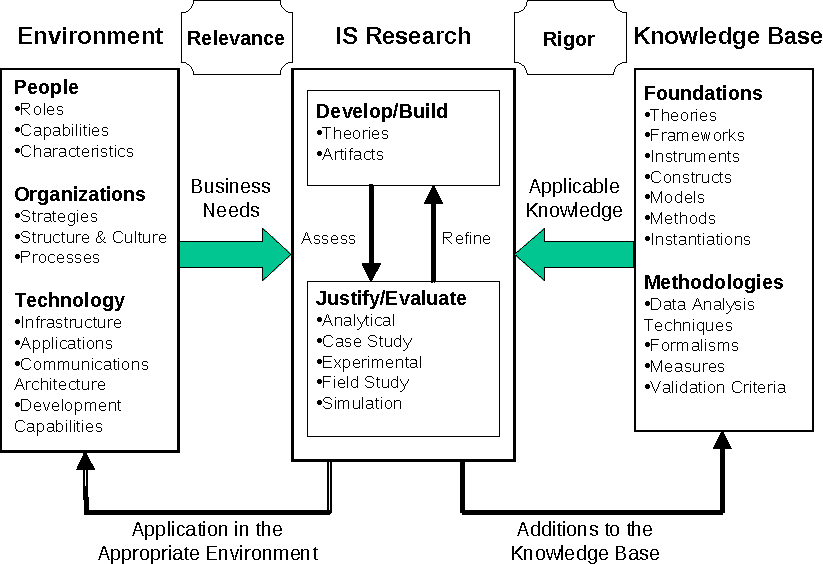
\includegraphics[width=1.0\textwidth]{figures/Hevner-et-al-2004-figure-2.pdf}
\caption{\label{fig:hevner}Information Systems Research Framework (Hevner et al 2004)}
\end{figure*}

Hevner et al (2004) defines seven guidelines that design-science in information systems should address (but not necessarily come-what-may adhere to), which will be done in the next chapter. % TODO more conrete/clickable reference
They are as follows:

% TODO
% \begin{leftbar}
%  asdf
%  asdf
%\begin{leftbar}

%\begin{siderules}
%\begin{quotation}
\begin{description}

\item[Design as an Artifact]
``Design-science research must produce a viable artifact in the form of a construct, a model, a method, or an instantiation.'' This allows to demonstrate feasibility -- for cases where that wasn't a given yet -- thus making it research (as opposed to routine design).

% This

\item[Problem Relevance]
``The objective of design-science research is to develop technology-based solutions to important and relevant business problems.'' Relevancy here is with respect to a  ``constituent community'' (e.g. IS practitioners)
% TODO mention Technology Acceptance Model here (and need to define it)? i haven't really done anything based on it, so whatever

\item[Design Evaluation]
``The utility, quality, and efficacy of a design artifact must be rigorously demonstrated via well-executed evaluation methods.'' This usually requires integration into the usage context (to see if it ``works'' there or is ``good'' in it), the definition of appropriate metrics and gathering of appropriate data. Evaluation provides valueable and necessary feedback for the design iterations (see figure \ref{fig:hevner})

\item[Research Contributions]
``Effective design-science research must provide clear and verifiable contributions in the areas of the design artifact, design foundations, and/or design methodologies.'' Important here is the novelty of the artifact -- by extending or innovatively (re-)applying previous knowledge -- as well as its generality and significance.

\item[Research Rigor]
``Design-science research relies upon the application of rigorous methods in both the construction and evaluation of the design artifact.'' This means applying existing foundations and methodologies, using effective metrics and formalising. Note, however, that an overemphasis on rigor can often lead to lower relevance (Lee 1999), as many environments and artifacts defy an excessive formalism (see ``wicked problems'' at footnote \ref{ref:wicked}). %TODO better reference / use glossary entry

\item[Design as a Search Process]
``The search for an effective artifact requires utilizing available means to reach desired ends while satisfying laws in the problem environment.'' This entails using heuristic search stragegies (e.g. best-practices as starting point) in ght generate/test-cycle (see figure \ref{fig:hevner}) However, again, it might not be possible to formalize or even determine any of these, due to the ``wicked'' (see footnote \ref{ref:wicked}) nature of tackled problems. As a result it might often be necessary to only work on simpler sub-problems, giving up relevancy in turn.

\item[Communication of Research]
``Design-science research must be presented effectively both to technology-oriented as well as management-oriented audiences.'' For the former the construction and evaluation process are important (e.g. to allow reproduction). For the latter the question boils down to ``Is it worth the effort to use the artifact for my business?''. This can be broken down as ``What knowledge is required?'' respectively ``Who can use it?'', ``How imporant is the problem?'', ``How effective is the solution?'' as well as some details in appendicesto appreciating the work.

\end{description}
%\end{quotation}
%\end{siderules}



\subsection{Design Evaluation Methods}

\begin{comment}
% TODO drop methods that weren't used

% TODO metrics from "Design Evaluation:"
  * evaluate in terms of:
    * functionality
    * completeness
    * consistency
    * accuracy
    * performance
    * reliability
    * usability
    * fit with the organization
    * other relevant quality attributes
* establish if it does work and in which environments
  * what constitutes “working” and “good”? which metrics?
  * compare with other solutions for the same problem by human experts
\end{comment}

Observational methods:

\begin{description}
  \item[Case Study] ``Study artifact in depth in business environment''
    % * **{** ^ that **}**
    % * **{** anecdotal evidence by fsu/fk/sbyim/yp how they feel about it? (super-biased due to interaction with me) **}**
  \item[Field Study] ``Monitor use of artifact in multiple projects''
    % * **{** the meinkauf app! what did we use there? ionic and vanilla angular or ng-redux too? <!-- TODO get copy of mk repo --> **}**
\end{description}

Analytical methods:

\begin{description}
  \item[Static Analysis] ``Examine structure of artifact for static qualities (e.g., complexity)''
    % * **{** graph out dependencies in both apps, if necessary in one vertical slice of one process <!-- TODO make graph of dependencies -->  **}**
    % * **{** code-examples of very simple apps with both architectures to demonstrate boiler-plate / overhead? Todo-MVC? <!-- TODO write examples -->  **}**
  \item[Architecture Analysis] ``Study fit of artifact into technical IS architecture''
    % * **{** analyze how well it interacts with the rest of the WoN-ecosystem. what defines “interacts well”? <!-- TODO ponder --> **}**
  \item[Optimization] ``Demonstrate inherent optimal properties of artifact or provide optimality bounds on artifact behavior''
  \item[Dynamic Analysis] ``Study artifact in use for dynamic qualities (e.g., performance)''
\end{description}

Experimental Methods:

\begin{description}
  \item[Controlled Experiment] ``Study artifact in controlled environment for qualities (e.g., usability)''
  \item[Simulation] ``Execute artifact with artificial data''
\end{description}

Testing:

\begin{description}
  \item[Functional (Black Box) Testing] ``Execute artifact interfaces to discover failures and identify defects''
  \item[Structural (White Box) Testing] ``Perform coverage testing of some metric (e.g., execution paths) in the artifact implementation''
\end{description}

Descriptive Methods:

\begin{description}
  \item[Informed Argument] ``Use information from the knowledge base (e.g., relevant research) to build a convincing argument for the artifact’s utility''
    % * **{** ^ this **}**
    % TODO: ^ (only) usable for more innovative artifacts for which other methods aren’t feasible
  \item[Scenarios] ``Construct detailed scenarios around the artifact to demonstrate its utility''
\end{description}





% See figure \ref{fig:hevner} \dots
